
\documentclass[pdf]{beamer}

\mode<presentation>{}

\usetheme{CambridgeUS}

\usepackage[utf8]{inputenc}
\usepackage{tikz}
\usetikzlibrary{positioning}
\usetikzlibrary{calc}

\usepackage{listings}
\lstset{emph={new, val, trait}, emphstyle=\color{red} }
\title{Tower Defense}
\author{Alexis Laouar, R\'emi Oudin, K\'evin Le Run}

\begin{document}

\begin{frame}
  \titlepage
\end{frame}

\section{Plus court chemin}

\begin{frame}
    \frametitle{Jump point search}
    Algorithme utilis\'e : Jump Point Search (JPS)\\
    A* o\`u l'on r\'eduit le nombre de noeuds ouverts en prenant en compte la
    direction de parcours
\end{frame}

\begin{frame}
    \begin{figure}[h]
        \centering
        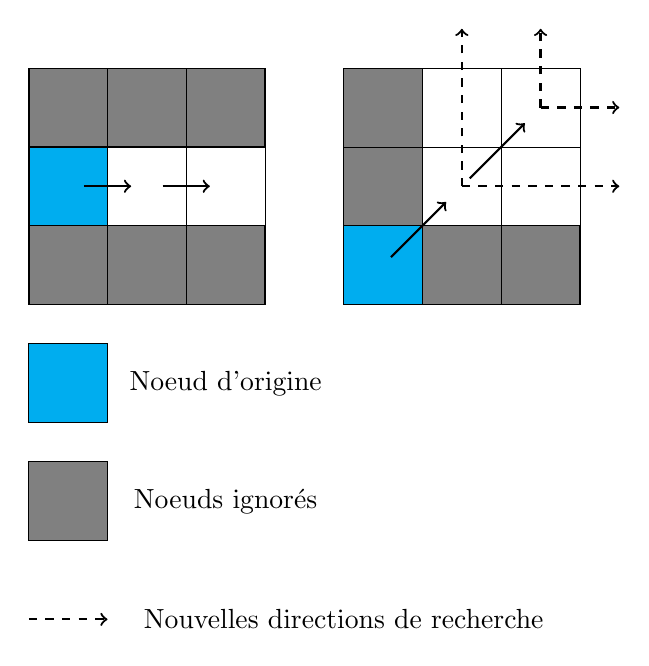
\begin{tikzpicture}
            \draw[fill=cyan] (0,1) rectangle (1,2);
            \draw[fill=gray] (0,0) rectangle (3,1);
            \draw[fill=gray] (0,2) rectangle (3,3);
            \draw[step=1cm,very thin] (0,0) grid (3,3);
            \draw[thick,->] (1.7,1.5) -- (2.3,1.5);
            \draw[thick,->] (0.7,1.5) -- (1.3,1.5);

            \draw[fill=cyan] (4,0) rectangle (5,1);
            \draw[fill=gray] (4,1) rectangle (5,3);
            \draw[fill=gray] (5,0) rectangle (7,1);
            \draw[step=1cm,very thin] (4,0) grid (7,3);
            \draw[thick,->] (4.6,0.6) -- (5.3,1.3);
            \draw[thick,->] (5.6,1.6) -- (6.3,2.3);
            \draw[thick,dashed,->] (5.5,1.5) -- (5.5,3.5);
            \draw[thick,dashed,->] (5.5,1.5) -- (7.5,1.5);
            \draw[thick,dashed,->] (6.5,2.5) -- (6.5,3.5);
            \draw[thick,dashed,->] (6.5,2.5) -- (7.5,2.5);

            \draw[black,fill=cyan] (0,-0.5) rectangle (1,-1.5);
            \node at (2.5,-1) {Noeud d'origine};
            \draw[black,fill=gray] (0,-2) rectangle (1,-3);
            \node at (2.5,-2.5) {Noeuds ignor\'es};
            \draw[dashed,thick,->] (0,-4) -- (1,-4);
            \node at (4,-4) {Nouvelles directions de recherche};
        \end{tikzpicture}
        \caption{Beaucoup de cases ignor\'ees}
    \end{figure}
\end{frame}

\begin{frame}
    \begin{figure}[h]
        \centering
        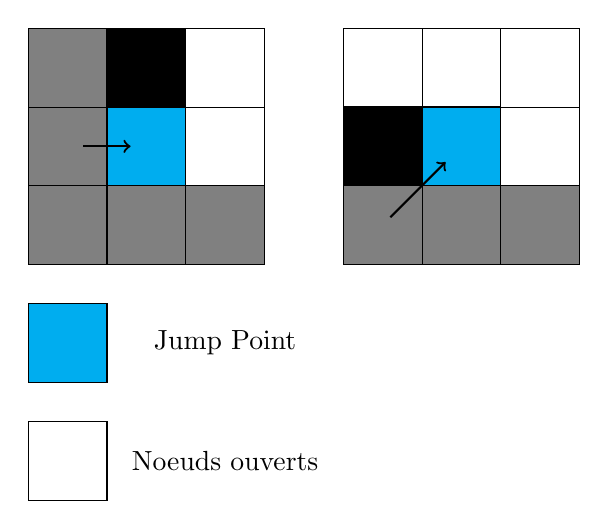
\begin{tikzpicture}
            \draw[fill=cyan] (1,1) rectangle (2,2);
            \draw[fill=gray] (0,0) rectangle (1,3);
            \draw[fill=gray] (1,0) rectangle (3,1);
            \draw[fill=black] (1,2) rectangle (2,3);
            \draw[step=1cm,very thin] (0,0) grid (3,3);
            \draw[thick,->] (0.7,1.5) -- (1.3,1.5);

            \draw[fill=cyan] (5,1) rectangle (6,2);
            \draw[fill=black] (4,1) rectangle (5,2);
            \draw[fill=gray] (4,0) rectangle (7,1);
            \draw[step=1cm,very thin] (4,0) grid (7,3);
            \draw[thick,->] (4.6,0.6) -- (5.3,1.3);

            \draw[black,fill=cyan] (0,-0.5) rectangle (1,-1.5);
            \node at (2.5,-1) {Jump Point};
            \draw[black] (0,-2) rectangle (1,-3);
            \node at (2.5,-2.5) {Noeuds ouverts};
        \end{tikzpicture}
        \caption{Les Jump Points}
    \end{figure}
\end{frame}

\end{document}
